\section{Propostas para Descoberta de Serviços} \label{sec:propostas-descoberta-ws}

Devido ao encerramento dos repositórios UDDI públicos, suportados pela W3C,  como apresentado na Seção \ref{sec:uddi} e mencionado em \cite{lausen2007finding} \cite{treiber2007active}, surgem novas propostas para descoberta de serviços, como \cite{lausen2007finding} \cite{wu2008novel} \cite{wu2009new} \cite{al2008toward} \cite{borges2007arquitetura}. Algumas delas serão apresentadas nas sub-seções seguintes.

\subsection{\textit{A Novel Interoperable Model of Distributed UDDI} \cite{wu2008novel}} \label{sec:novel-model-uddi}

Segundo \cite{wu2008novel}, a maioria dos modelos de UDDI são centralizados, o que pode acarretar perda de performance caso existam muitos serviços para serem registrados ou pesquisados. Tal arquitetura centralizado não possui tolerância a falhas e não permite balanceamento de carga. Outro problema de tais modelos é a falta de detecção ativa de mudanças em \textit{Web Services} e captura de falhas, impedindo que seja informado aos clientes que um determinado serviço não está funcional.

Em \cite{wu2008novel} é apresentada uma arquitetura distribuída para repositórios UDDI, sendo composta de servidores raiz, super servidores de domínio e servidores normais, descritos a seguir. 

Os servidores raiz são um grupo de servidores, semelhantes a servidores raízes DNS, podendo ser um ou mais. Eles não realizam busca e publicação de serviços, apenas registram informações dos super servidores de domínio e proveem a função de registro e busca por este tipo de servidor para compor o repositório UDDI.

Os super servidores de domínio são responsáveis pelo gerenciamento dos servidores normais mais próximos, e proveem registro e busca de serviços, além de poderem obter informações relacionadas de outros super servidores de domínio, a partir dos servidores raiz, para obter mais informações de serviços.

Os servidores normais são usados para permitir aos usuários, publicarem e buscarem por informações de serviços. Eles enviam requisições de busca aos super servidores de domínio se não existir nenhum serviço adequado. A Figura \ref{fig:distributed-uddi} apresenta a arquitetura da proposta.

\begin{center}
	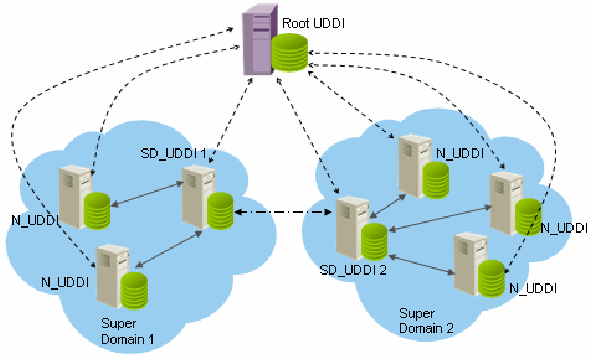
\includegraphics[scale=0.6]{images/a-novel-interoperable-model-uddi.png}
	\captionof{figure}{Arquitetura Distribuída de Repositório UDDI \cite{wu2008novel}}
	\label{fig:distributed-uddi}
\end{center}

Alguns dos objetivos desta arquitetura são: permitir registrar informações sobre os serviços que se tornaram inativos e reduzir o tempo de resposta na busca de serviços. Os autores declarem ter atingido tais objetivos.


